\documentclass[11pt,a4paper]{article}

% Pacchetti fondamentali
\usepackage[utf8]{inputenc}
\usepackage[italian]{babel}
\usepackage{amsmath}
\usepackage{graphicx}
\usepackage{geometry}
\usepackage{booktabs}
\usepackage{float}
\usepackage{hyperref}
\usepackage{caption}
\usepackage{longtable}

% Margini del testo ripristinati a 2.5cm (standard accademico)
\geometry{a4paper, top=2.5cm, bottom=2.5cm, left=2.5cm, right=2.5cm}

\title{\textbf{Analisi delle Prestazioni di Modelli Centralizzati ILP per il Task Offloading}}
\author{Claudio Bagini 2045337}
\date{\today}

\begin{document}

\maketitle

\section{Introduzione}
Nel contesto dei sistemi distribuiti moderni e dell'edge computing, l'allocazione efficiente delle risorse computazionali (Resource Allocation) e l'istradamento dei task (Task Routing) rappresentano sfide critiche e di primaria importanza. 

Il sistema analizzato in questo studio sfrutta un approccio centralizzato basato su Integer Linear Programming (ILP) per mappare le richieste in ingresso sui nodi server disponibili. A differenza delle euristiche, che compiono scelte ottime a livello puramente locale (ma spesso sub-ottime a livello globale), il modello ILP garantisce l'individuazione di una soluzione matematicamente perfetta per un dato set di richieste.

Per comprendere a fondo l'impatto delle policy di orchestrazione e il comportamento del solutore centralizzato sotto stress, il modello è stato testato imponendo due diverse strategie di mappatura (\textit{Objective Mapping}) nella funzione obiettivo:
\begin{itemize}
    \item \textbf{Mapping Time:} I pesi della funzione obiettivo privilegiano la minimizzazione del tempo totale di risposta e di trasmissione ($W_{lat}=1, W_{en}=0$). Questa strategia è cruciale per i servizi altamente sensibili al ritardo (delay-sensitive).
    \item \textbf{Mapping Energy:} I pesi della funzione obiettivo privilegiano il risparmio energetico dei nodi e della rete ($W_{lat}=0, W_{en}=1$), parametro fondamentale per estendere la vita operativa di infrastrutture con rigidi vincoli di power-budget.
\end{itemize}
Le simulazioni mirano a individuare i colli di bottiglia fisici e logici del sistema e a valutare quali configurazioni di \textit{Batch Size} (dimensione della coda di richieste aggregata) e \textit{Batch Timeout} (tempo massimo di attesa prima di innescare l'ILP) garantiscano la maggiore resilienza al variare del tasso di arrivo delle richieste nella rete.

\section{Setup Sperimentale}
Le simulazioni sono state eseguite mantenendo un set di parametri di base costanti (ispirati al paper ICDCS di riferimento), al fine di isolare l'impatto delle metriche di interesse.

\subsection{Parametri e Variabili dell'Esperimento}
\begin{itemize}
    \item \textbf{Budget Energetico Globale:} Fissato rigorosamente a 80 KJ per l'intera durata di ogni iterazione di simulazione.
    \item \textbf{Arrival Rate (Carico di Rete):} Variabile indipendente principale. Il tasso di arrivo delle richieste è stato modulato per simulare scenari di traffico progressivo: da 2, 3, 4, 6, 8 fino a 10 richieste al secondo. Nel motore del simulatore, questi valori corrispondono a tempi di inter-arrivo (\textit{AT}) decrescenti (da $0.5$ a $0.1$ secondi).
    \item \textbf{Configurazioni di Batching:} Per ogni livello di \textit{Arrival Rate}, sono state testate molteplici configurazioni incrociate. Variando la \textit{Batch Size} (BS), si è stabilito quante richieste accumulare prima di avviare il solutore ILP (da 1 a 20). Variando il \textit{Batch Timeout} (BT), si è imposto un limite temporale massimo per prevenire lo stallo delle richieste (starvation) in scenari di traffico rado.
    \item \textbf{Coefficienti di Ponderazione ($\alpha$, $\beta$, $\gamma$):} In stretta conformità con il modello matematico del paper di riferimento, i vettori dei pesi che regolano i trade-off e i costi delle risorse all'interno della formulazione ILP sono stati mantenuti costanti, garantendo la coerenza dell'esperimento. Nello specifico, i parametri di profilazione sono stati fissati ai seguenti valori vettoriali: $\alpha = (0.3, 0.5, 0.2)$, $\beta = (0.4, 0.35, 0.25)$ e $\gamma = (0.7, 0.3)$.
\end{itemize}


\section{Analisi dei Risultati}
Di seguito vengono presentati e discussi i risultati per le tre metriche cardine: Success Rate, Cause di Rigetto e Response Time.

\subsection{Success Rate (Tasso di Completamento)}
Il tasso di successo rappresenta la percentuale di task che sono stati correttamente presi in carico, elaborati e restituiti all'utente senza violare la deadline e il budget energetico.

\begin{figure}[H]
    % \makebox e 1.15\textwidth permettono all'immagine di espandersi oltre i margini del testo!
    \makebox[\textwidth][c]{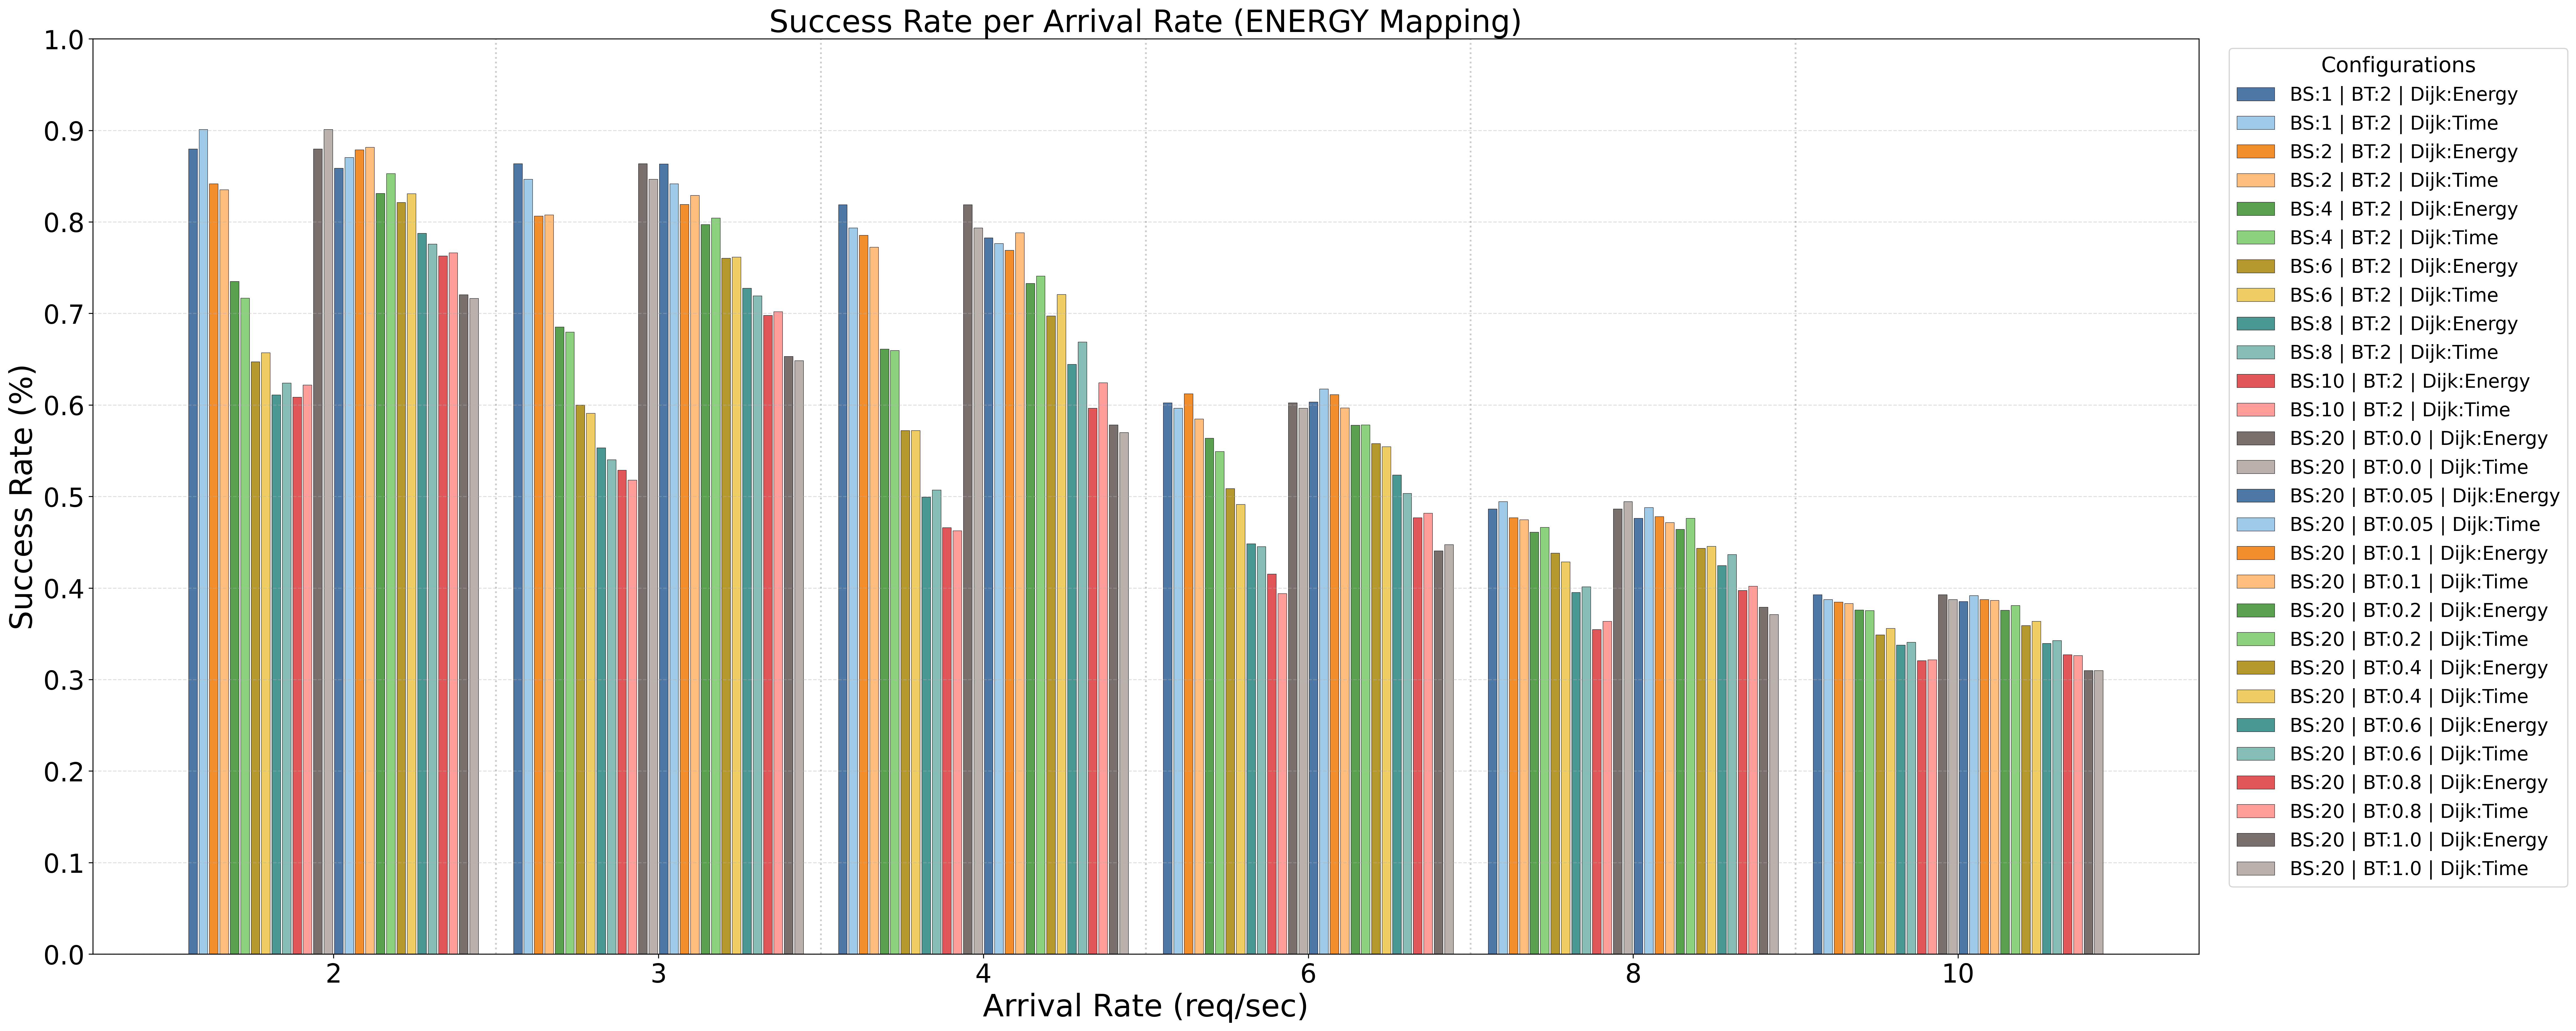
\includegraphics[width=1.3\textwidth]{01_AR_success_rate_energy.png}}
    \caption{Success Rate - Configurazione Energy.}
    \label{fig:suc_energy}
\end{figure}

\begin{figure}[H]
    \makebox[\textwidth][c]{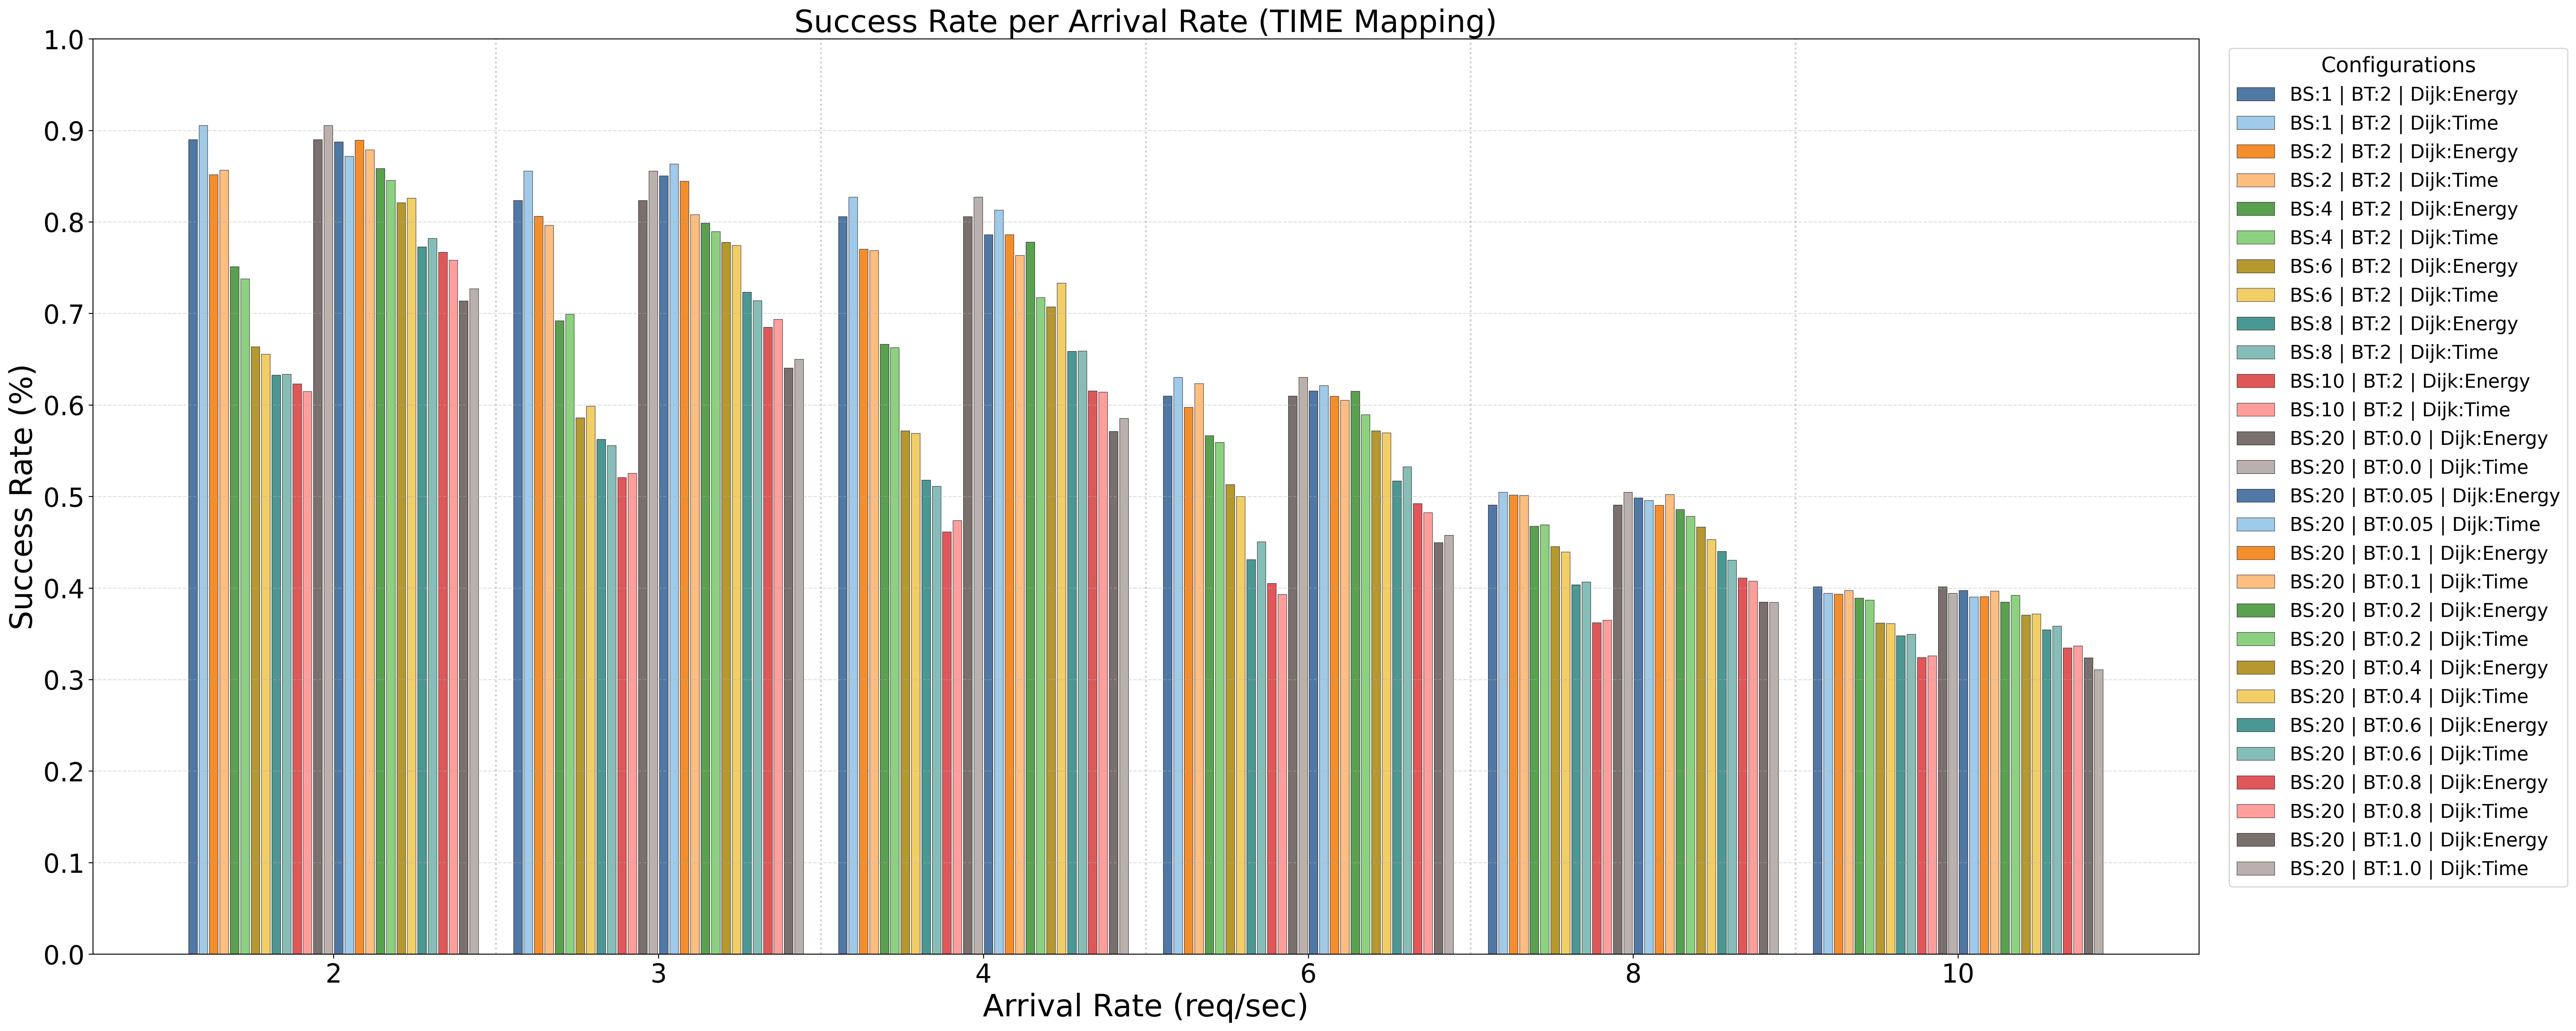
\includegraphics[width=1.3\textwidth]{01_AR_success_rate_time.png}}
    \caption{Success Rate - Configurazione Time.}
    \label{fig:suc_time}
\end{figure}

Come visibile nelle Figure \ref{fig:suc_energy} e \ref{fig:suc_time}, il sistema mostra una tenuta eccellente per carichi leggeri (fino a 4 richieste al secondo). Superata la soglia critica delle 6 req/sec, si osserva un declino delle prestazioni. L'elemento cruciale nel mitigare tale degrado risiede tuttavia nella riduzione del parametro \textit{Batch Timeout} (BT). Le configurazioni caratterizzate da un timeout estremamente contenuto (visibili nei blocchi sulla destra per ciascun Arrival Rate) mantengono tassi di successo sensibilmente superiori sotto forte stress. 
\subsection{Analisi delle Cause di Rigetto (Rejection Causes)}
Per diagnosticare con esattezza la causa del collasso prestazionale, i task scartati sono stati analizzati in base allo stato di fallimento registrato.

\begin{figure}[H]
    \makebox[\textwidth][c]{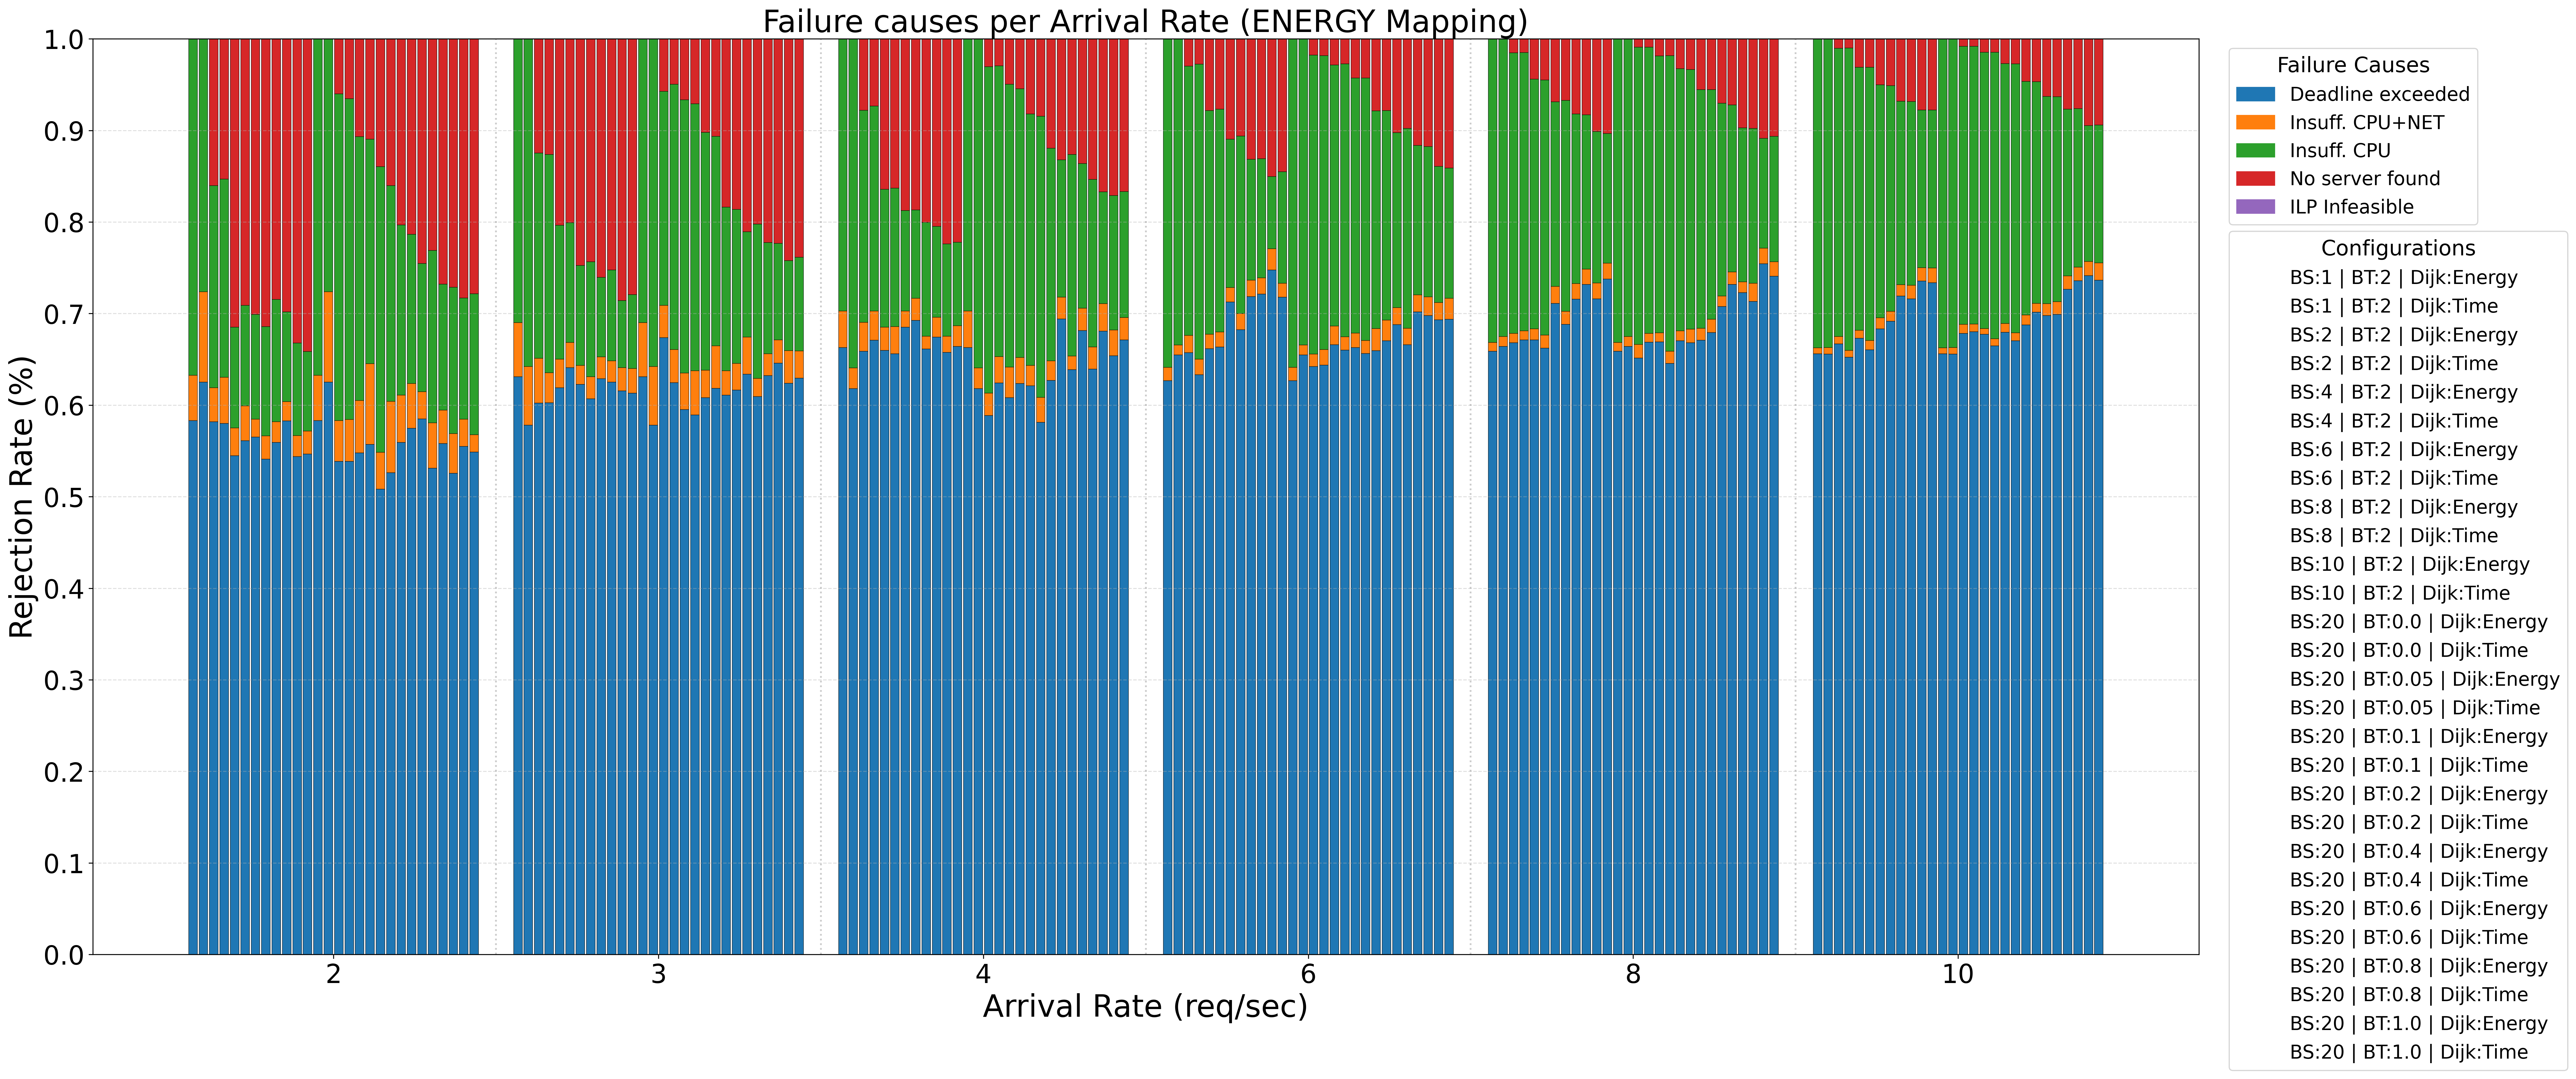
\includegraphics[width=1.3\textwidth]{02_AR_rejection_energy.png}}
    \caption{Distribuzione delle Cause di Rigetto sul totale dei task (Configurazione Energy).}
        \label{fig:rej_energy}
\end{figure}

\begin{figure}[H]
    \makebox[\textwidth][c]{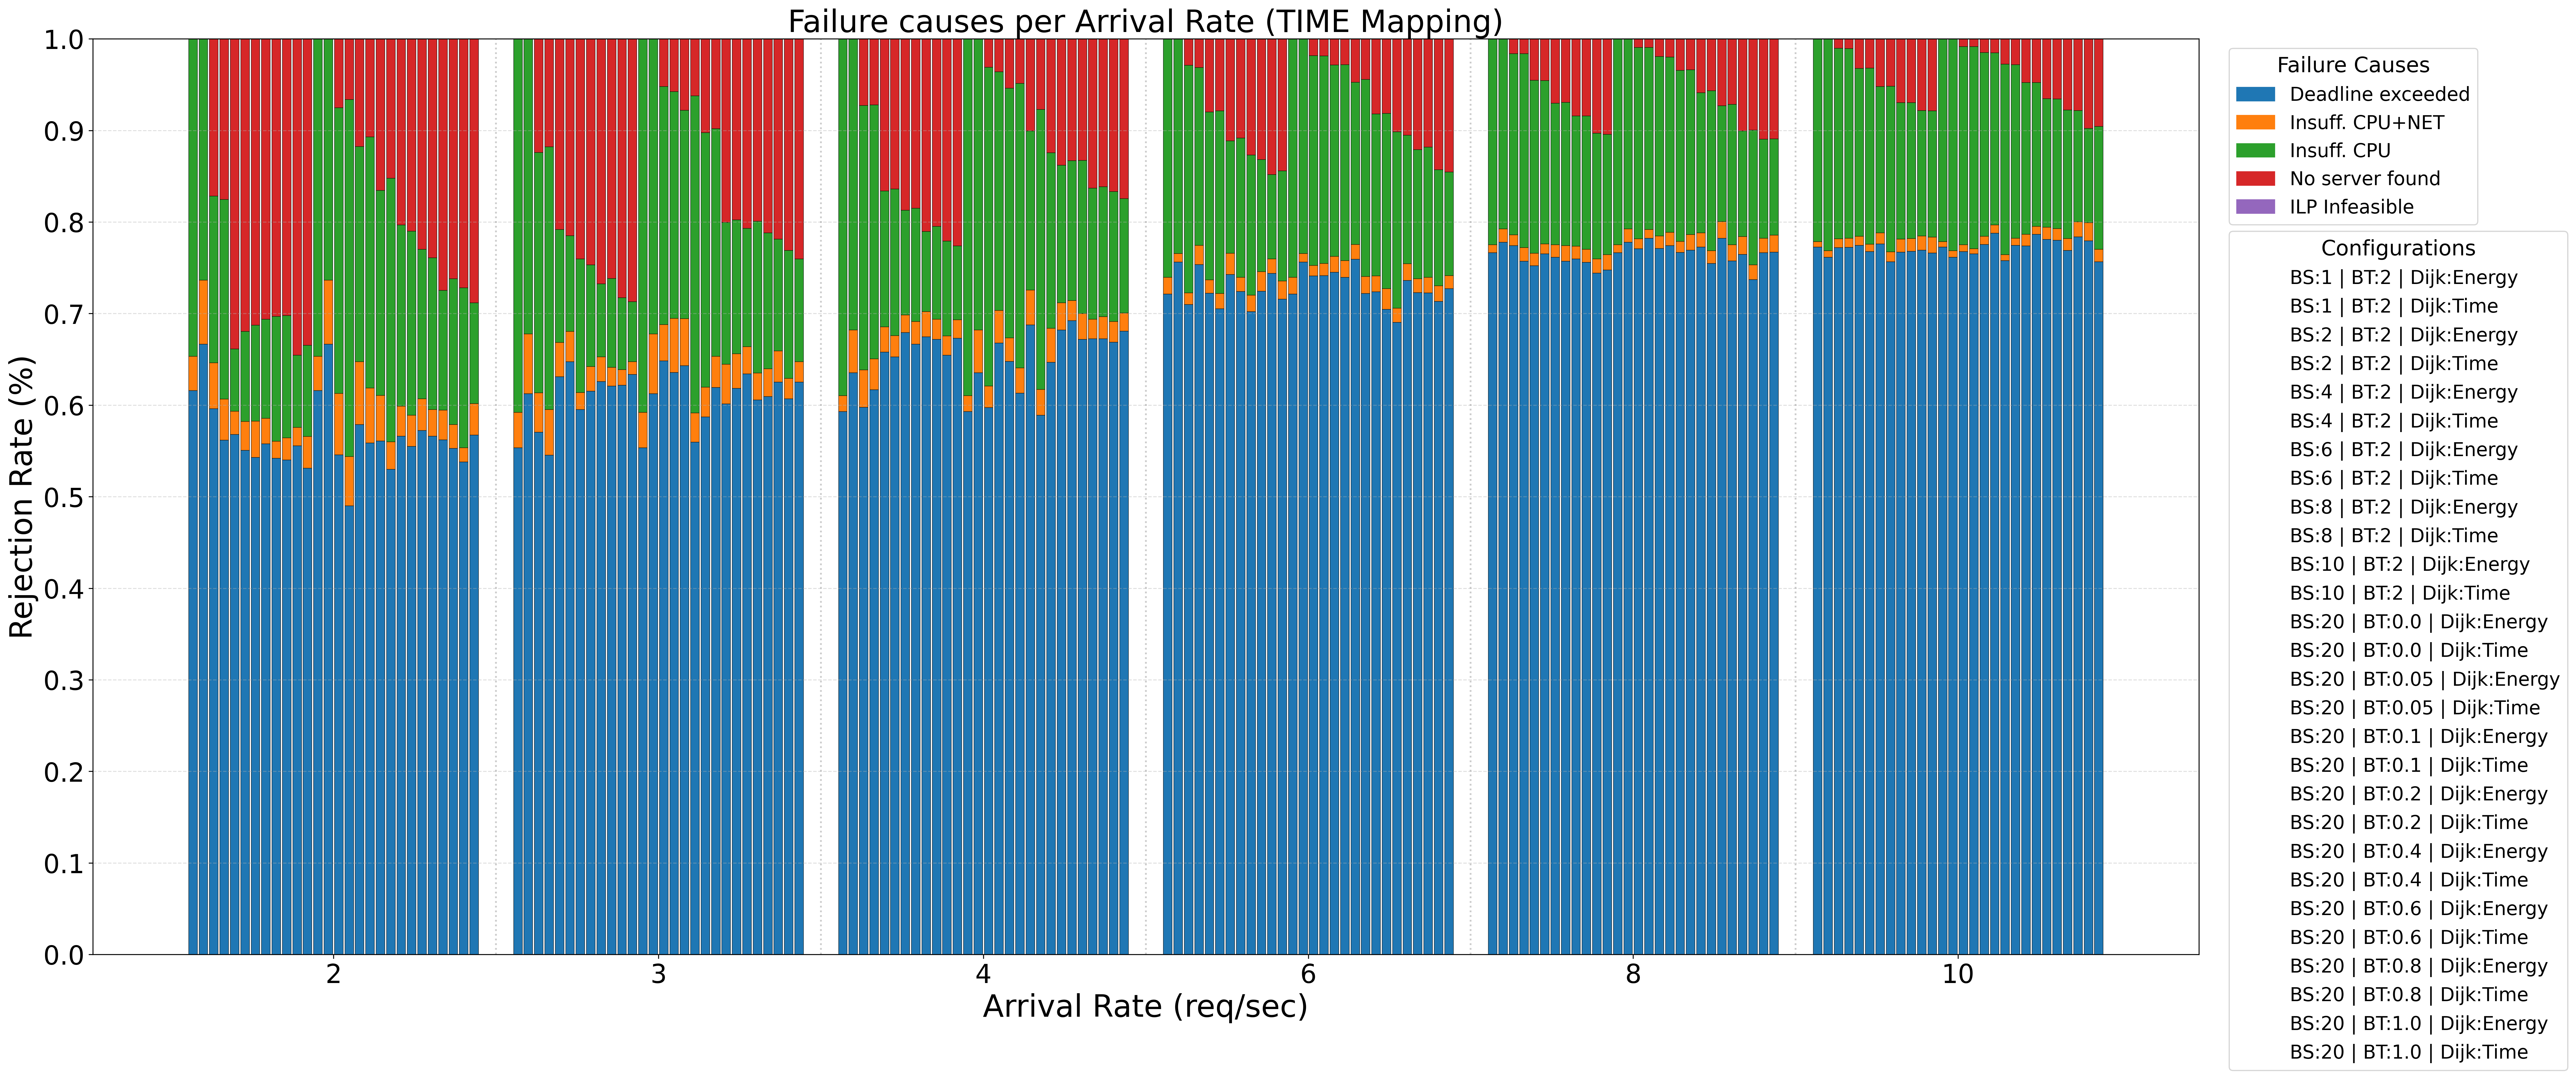
\includegraphics[width=1.3\textwidth]{02_AR_rejection_time.png}}
    \caption{Distribuzione delle Cause di Rigetto sul totale dei task (Configurazione Time).}
    \label{fig:rej_time}
\end{figure}

Le Figure \ref{fig:rej_energy} e \ref{fig:rej_time} rivelano chiaramente la natura del collo di bottiglia. La causa schiacciante e predominante che porta al rigetto dei task è il \textbf{Deadline Exceeded}. All'aumentare estremo del carico, le violazioni delle scadenze monopolizzano di fatto i fallimenti dell'infrastruttura. In questo scenario, la configurazione "Time" (Figura \ref{fig:rej_time}) riesce a mitigare lievemente l'insorgenza delle deadline violation rispetto alla variante "Energy".
\subsection{Scomposizione del Tempo di Risposta (Response Time)}
L'ultima fase si concentra sul disaggregare il tempo di risposta totale nella componente di calcolo (\textit{System Execution}) e in quella di accodamento/instradamento (\textit{Network/Wait Time}).

\begin{figure}[H]
    \makebox[\textwidth][c]{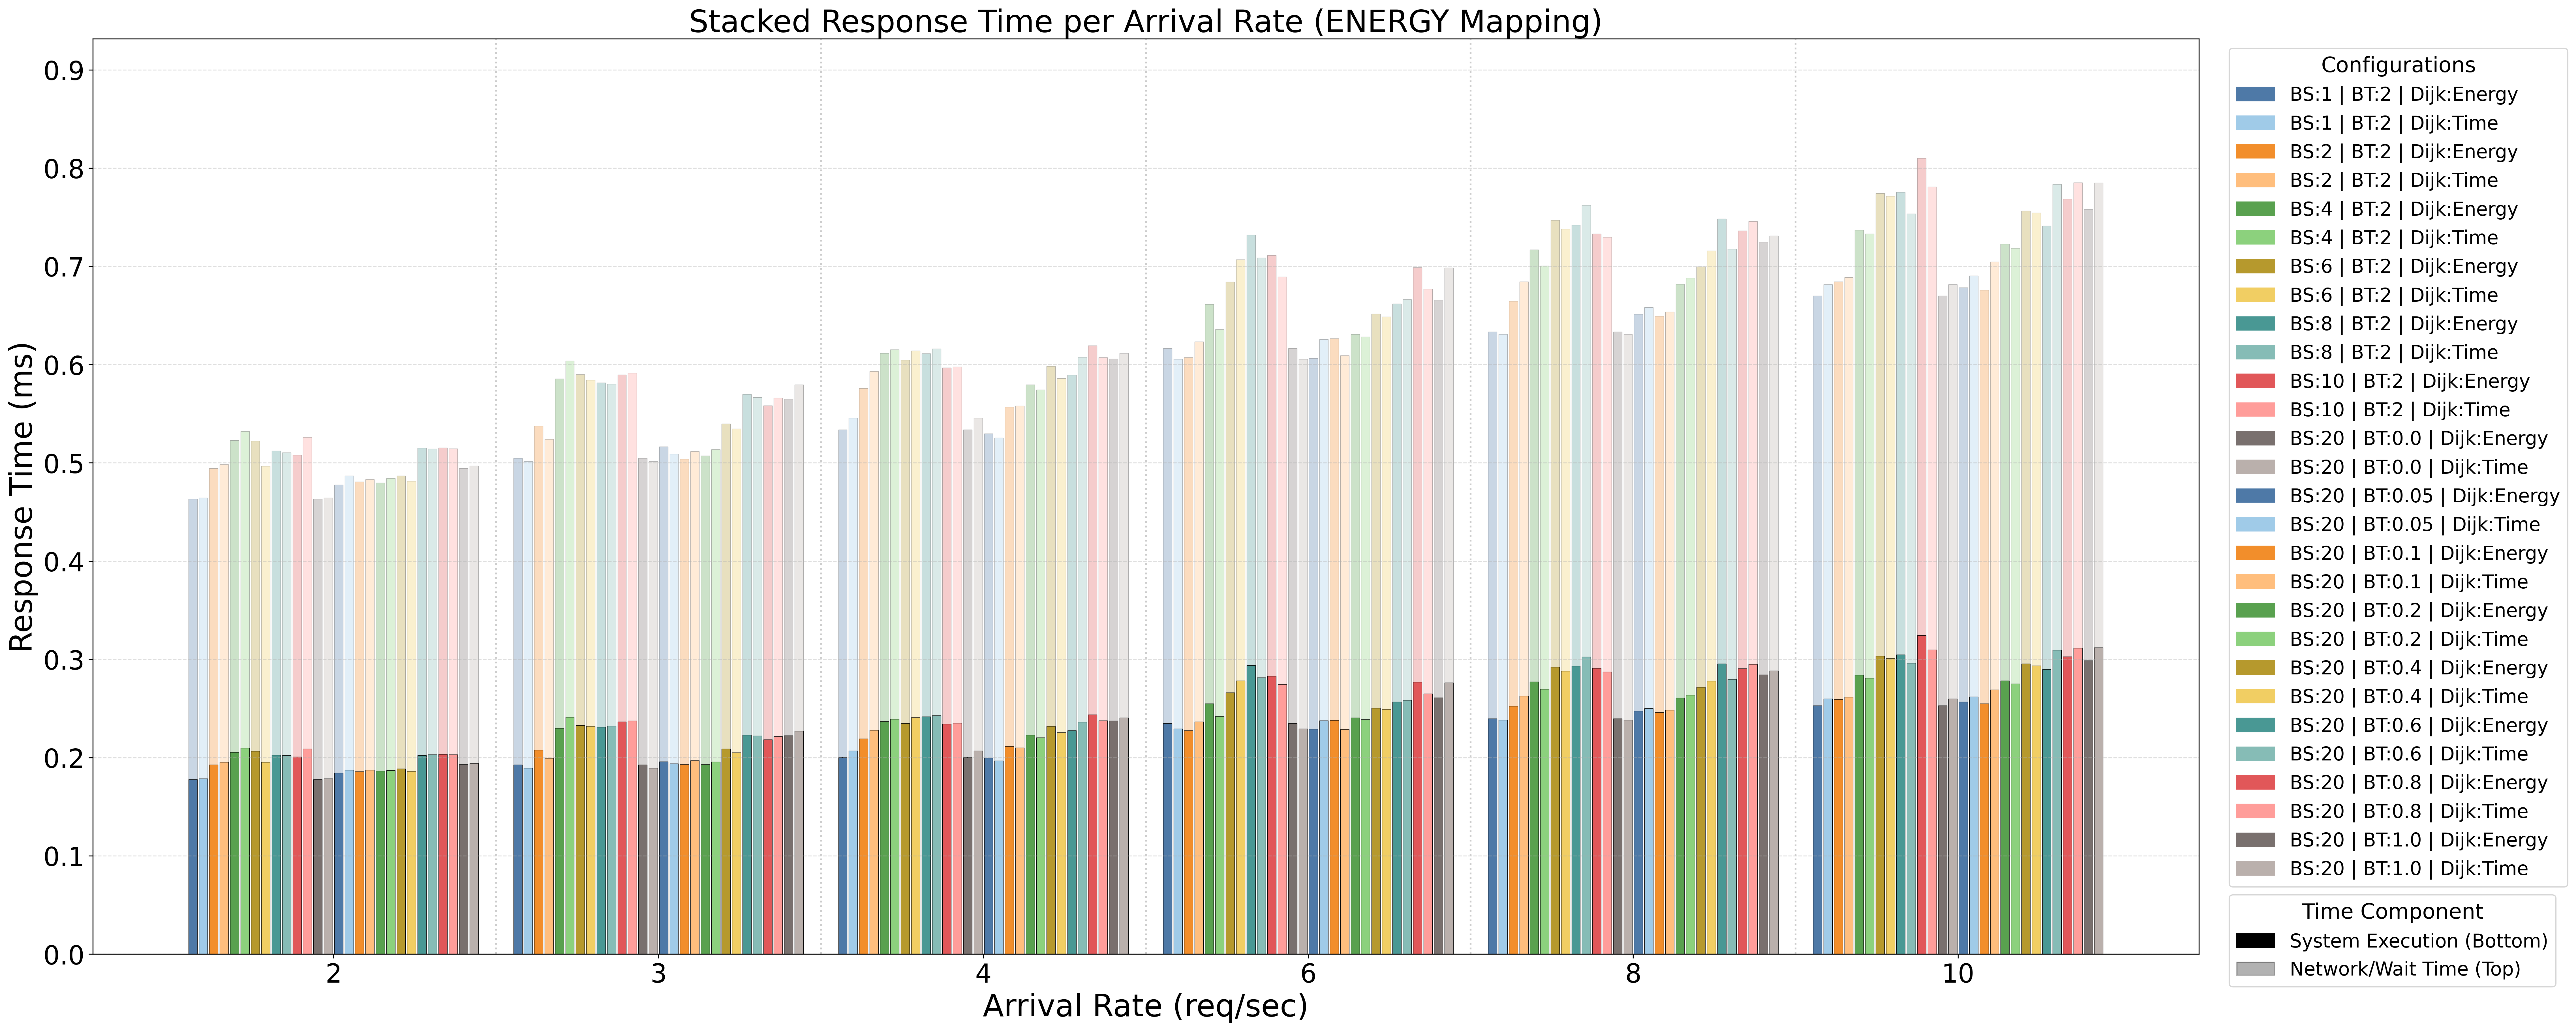
\includegraphics[width=1.3\textwidth]{03_AR_response_energy.png}}
    \caption{Scomposizione del Response Time (Configurazione Energy).}
    \label{fig:response_energy}
\end{figure}

\begin{figure}[H]
    \makebox[\textwidth][c]{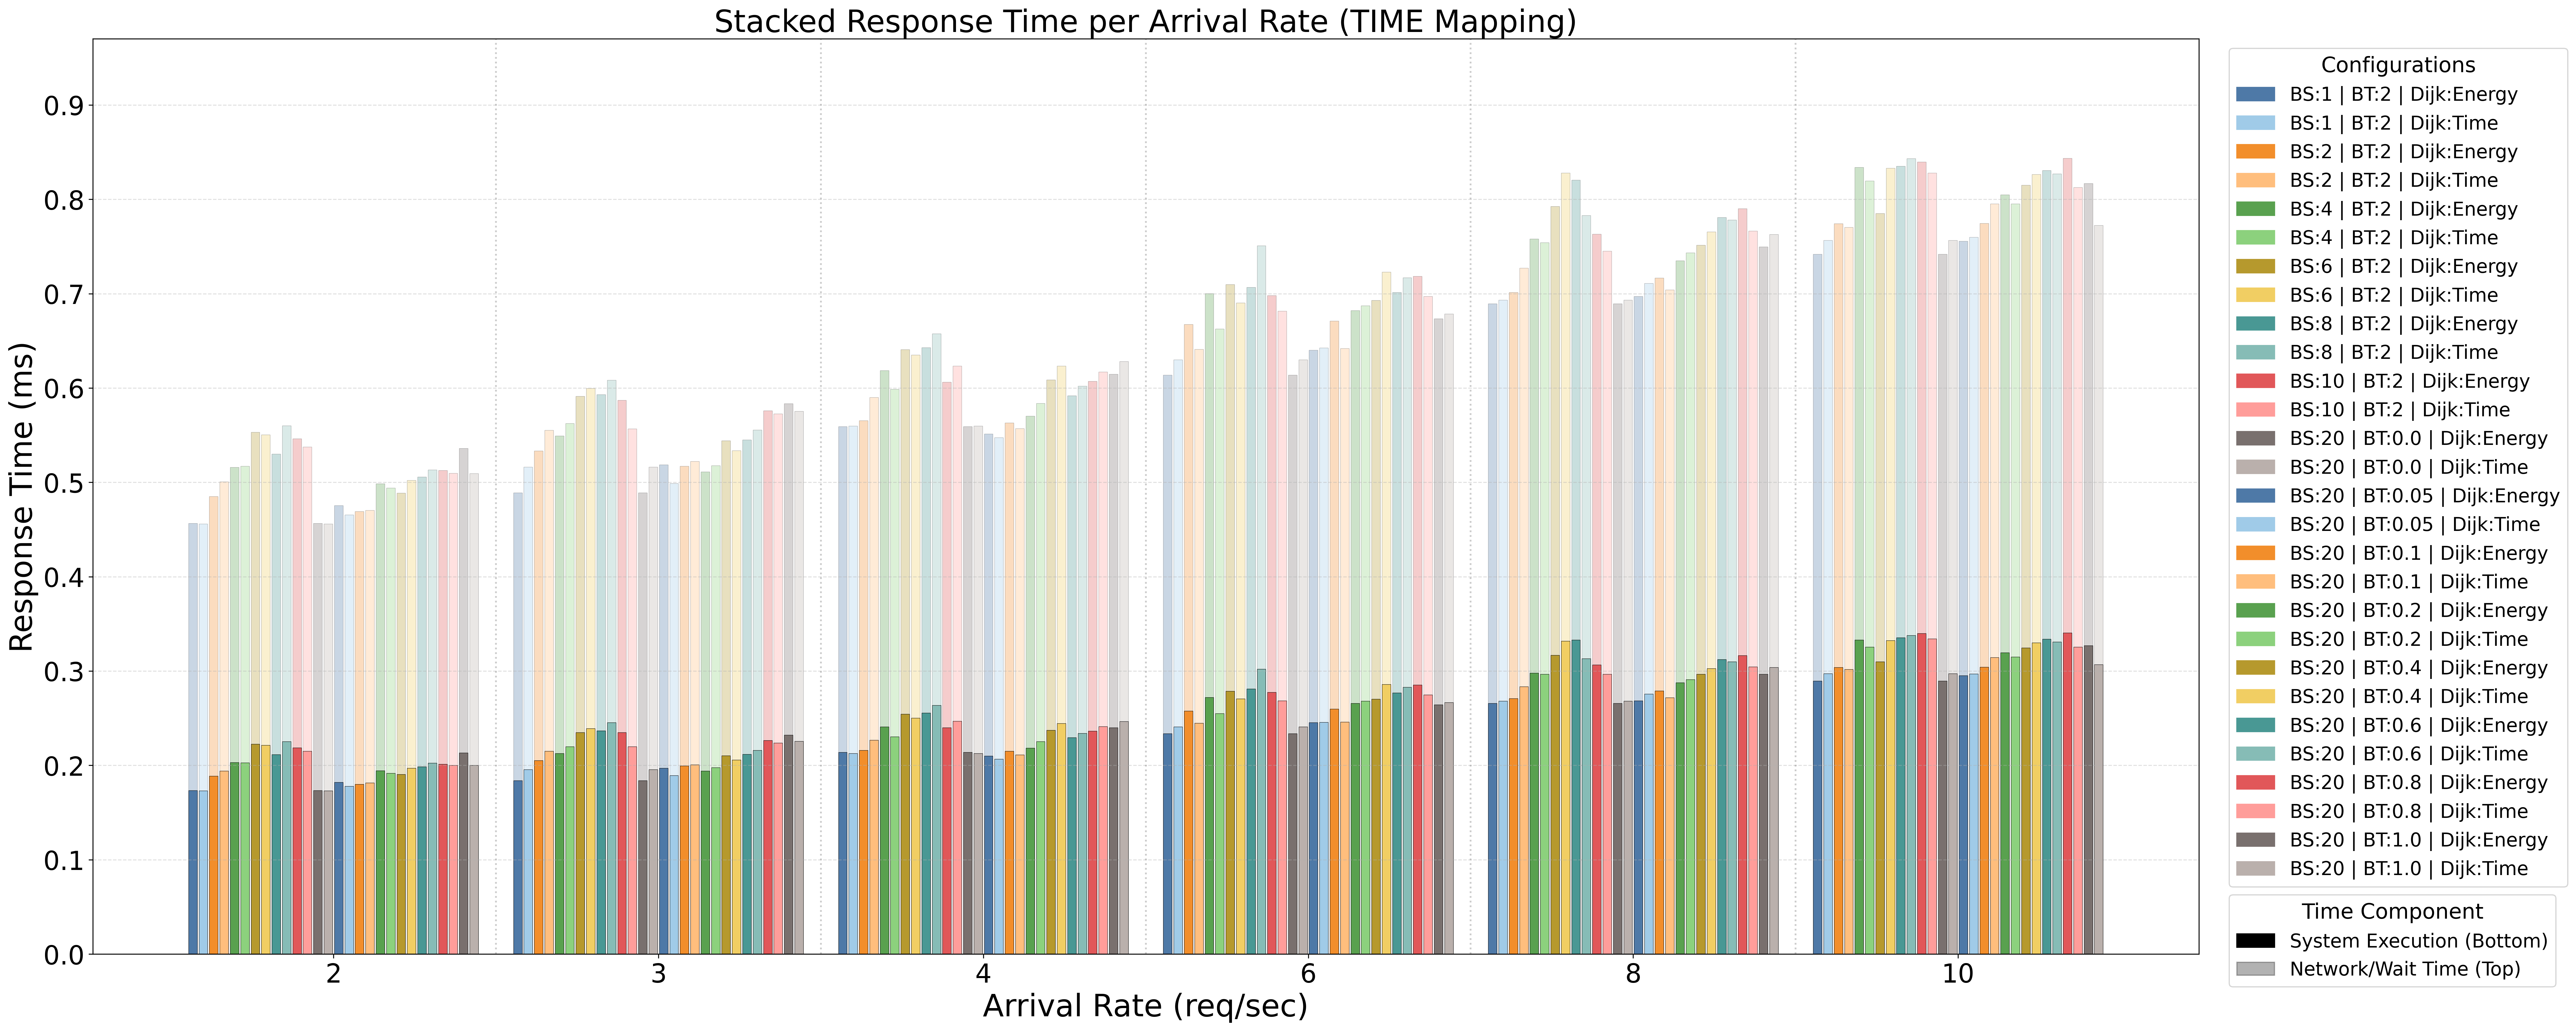
\includegraphics[width=1.3\textwidth]{03_AR_response_time.png}}
    \caption{Scomposizione del Response Time (Configurazione Time).}
    \label{fig:response_time}
\end{figure}

Le Figure \ref{fig:response_energy} e \ref{fig:response_time} illustrano con chiarezza la causa alla base della netta prevalenza dei rigetti per "Deadline Exceeded". Conformemente ai fondamenti della teoria delle code, man mano che il tasso di arrivo delle richieste ($\lambda$) si avvicina alla capacità massima di servizio del sistema ($\mu$), il tempo di attesa cresce in modo asintotico. Osservando i grafici, è evidente come il tempo di calcolo effettivo dei task (rappresentato dalle porzioni inferiori nere e piene) rimanga del tutto invariato. Al contrario, la latenza dovuta all'accodamento (evidenziata in grigio trasparente) subisce un incremento drastico in condizioni di alto carico
\section{Conclusioni}
L'analisi sperimentale ha convalidato la solidità dell'orchestrazione centralizzata ILP in contesti a carico medio-basso. L'utilizzo strutturato del Batching e del Timeout si è rivelato la scelta architetturale più impattante: accumulare richieste destabilizza l'algoritmo. I dati riassuntivi dell'intera simulazione sono aggregati nella Tabella \ref{tab:summary_csv}.

\section{Dati Sperimentali}

\begin{longtable}{ccccccc}
\caption{Tabella Riassuntiva: Valori medi (aggregati per Batch Size e Batch Timeout) al variare dell'Arrival Rate.} \label{tab:summary_csv} \\
\toprule
\textbf{Batch} & \textbf{Batch} & \textbf{Arrival} & \textbf{Success} & \textbf{Rej.} & \textbf{Rej.} & \textbf{Avg Total} \\
\textbf{Size} & \textbf{Timeout} & \textbf{Rate} & \textbf{Rate (\%)} & \textbf{Deadline (\%)} & \textbf{CPU (\%)} & \textbf{Resp. (ms)} \\
\midrule
\endfirsthead

\multicolumn{7}{c}%
{{\bfseries Tabella \thetable\ continuazione dalla pagina precedente}} \\
\toprule
\textbf{Batch} & \textbf{Batch} & \textbf{Arrival} & \textbf{Success} & \textbf{Rej.} & \textbf{Rej.} & \textbf{Avg Total} \\
\textbf{Size} & \textbf{Timeout} & \textbf{Rate} & \textbf{Rate (\%)} & \textbf{Deadline (\%)} & \textbf{CPU (\%)} & \textbf{Resp. (ms)} \\
\midrule
\endhead

\midrule
\multicolumn{7}{r}{{Continua nella pagina successiva...}} \\
\endfoot

\bottomrule
\endlastfoot

        1 & 2.0 & 2 & 89.41\% & 6.57\% & 3.36\% & 0.460 ms \\
        1 & 2.0 & 3 & 84.74\% & 9.02\% & 5.38\% & 0.503 ms \\
        1 & 2.0 & 4 & 81.14\% & 11.82\% & 6.46\% & 0.550 ms \\
        1 & 2.0 & 6 & 60.97\% & 26.86\% & 11.64\% & 0.616 ms \\
        1 & 2.0 & 8 & 49.41\% & 36.25\% & 13.80\% & 0.662 ms \\
        1 & 2.0 & 10 & 39.40\% & 43.10\% & 17.10\% & 0.713 ms \\
        \midrule
        2 & 2.0 & 2 & 84.63\% & 8.92\% & 3.22\% & 0.495 ms \\
        2 & 2.0 & 3 & 80.42\% & 11.35\% & 4.96\% & 0.538 ms \\
        2 & 2.0 & 4 & 77.43\% & 14.34\% & 5.78\% & 0.581 ms \\
        2 & 2.0 & 6 & 60.45\% & 27.18\% & 10.52\% & 0.635 ms \\
        2 & 2.0 & 8 & 48.86\% & 36.64\% & 13.11\% & 0.694 ms \\
        2 & 2.0 & 10 & 38.97\% & 43.67\% & 16.21\% & 0.730 ms \\
        \midrule
        4 & 2.0 & 2 & 73.53\% & 14.72\% & 2.58\% & 0.522 ms \\
        4 & 2.0 & 3 & 68.92\% & 19.73\% & 3.94\% & 0.575 ms \\
        4 & 2.0 & 4 & 66.25\% & 22.16\% & 5.15\% & 0.611 ms \\
        4 & 2.0 & 6 & 55.96\% & 30.30\% & 9.59\% & 0.665 ms \\
        4 & 2.0 & 8 & 46.61\% & 38.04\% & 12.28\% & 0.733 ms \\
        4 & 2.0 & 10 & 38.19\% & 44.41\% & 14.88\% & 0.781 ms \\
        \midrule
        6 & 2.0 & 2 & 65.59\% & 18.99\% & 3.85\% & 0.531 ms \\
        6 & 2.0 & 3 & 59.39\% & 24.78\% & 5.00\% & 0.591 ms \\
        6 & 2.0 & 4 & 57.12\% & 29.20\% & 4.76\% & 0.624 ms \\
        6 & 2.0 & 6 & 50.33\% & 35.53\% & 7.86\% & 0.698 ms \\
        6 & 2.0 & 8 & 43.78\% & 41.00\% & 10.46\% & 0.776 ms \\
        6 & 2.0 & 10 & 35.70\% & 46.74\% & 13.55\% & 0.791 ms \\
        \midrule
        8 & 2.0 & 2 & 62.53\% & 20.85\% & 4.70\% & 0.528 ms \\
        8 & 2.0 & 3 & 55.30\% & 27.95\% & 4.06\% & 0.591 ms \\
        8 & 2.0 & 4 & 50.89\% & 32.93\% & 5.06\% & 0.632 ms \\
        8 & 2.0 & 6 & 44.38\% & 39.86\% & 7.48\% & 0.725 ms \\
        8 & 2.0 & 8 & 40.17\% & 44.31\% & 9.60\% & 0.777 ms \\
        8 & 2.0 & 10 & 34.39\% & 48.72\% & 11.46\% & 0.802 ms \\
        \midrule
        10 & 2.0 & 2 & 61.71\% & 20.84\% & 3.51\% & 0.529 ms \\
        10 & 2.0 & 3 & 52.34\% & 29.60\% & 3.55\% & 0.581 ms \\
        10 & 2.0 & 4 & 46.59\% & 35.38\% & 5.04\% & 0.606 ms \\
        10 & 2.0 & 6 & 40.19\% & 43.74\% & 6.20\% & 0.695 ms \\
        10 & 2.0 & 8 & 36.14\% & 47.04\% & 9.20\% & 0.743 ms \\
        10 & 2.0 & 10 & 32.30\% & 50.86\% & 10.49\% & 0.815 ms \\
        \midrule
        20 & 0.0 & 2 & 89.41\% & 6.57\% & 3.36\% & 0.460 ms \\
        20 & 0.0 & 3 & 84.74\% & 9.02\% & 5.38\% & 0.503 ms \\
        20 & 0.0 & 4 & 81.14\% & 11.82\% & 6.46\% & 0.550 ms \\
        20 & 0.0 & 6 & 60.97\% & 26.86\% & 11.64\% & 0.616 ms \\
        20 & 0.0 & 8 & 49.41\% & 36.25\% & 13.80\% & 0.662 ms \\
        20 & 0.0 & 10 & 39.40\% & 43.10\% & 17.10\% & 0.713 ms \\
        \midrule
        20 & 0.05 & 2 & 87.20\% & 6.76\% & 4.52\% & 0.476 ms \\
        20 & 0.05 & 3 & 85.47\% & 9.37\% & 3.77\% & 0.511 ms \\
        20 & 0.05 & 4 & 78.96\% & 13.00\% & 6.79\% & 0.539 ms \\
        20 & 0.05 & 6 & 61.43\% & 26.67\% & 10.66\% & 0.629 ms \\
        20 & 0.05 & 8 & 48.96\% & 36.62\% & 13.38\% & 0.680 ms \\
        20 & 0.05 & 10 & 39.12\% & 44.00\% & 15.90\% & 0.721 ms \\
        \midrule
        20 & 0.1 & 2 & 88.21\% & 6.60\% & 3.08\% & 0.476 ms \\
        20 & 0.1 & 3 & 82.51\% & 10.40\% & 5.14\% & 0.514 ms \\
        20 & 0.1 & 4 & 77.67\% & 13.90\% & 6.63\% & 0.559 ms \\
        20 & 0.1 & 6 & 60.58\% & 27.70\% & 9.93\% & 0.637 ms \\
        20 & 0.1 & 8 & 48.56\% & 36.72\% & 13.09\% & 0.681 ms \\
        20 & 0.1 & 10 & 39.03\% & 44.27\% & 15.32\% & 0.738 ms \\
        \midrule
        20 & 0.2 & 2 & 84.70\% & 8.11\% & 4.09\% & 0.489 ms \\
        20 & 0.2 & 3 & 79.74\% & 12.33\% & 5.14\% & 0.512 ms \\
        20 & 0.2 & 4 & 74.24\% & 15.89\% & 6.94\% & 0.577 ms \\
        20 & 0.2 & 6 & 59.02\% & 28.64\% & 9.88\% & 0.657 ms \\
        20 & 0.2 & 8 & 47.62\% & 37.62\% & 12.30\% & 0.712 ms \\
        20 & 0.2 & 10 & 38.34\% & 44.41\% & 15.06\% & 0.760 ms \\
        \midrule
        20 & 0.4 & 2 & 82.49\% & 9.88\% & 3.28\% & 0.490 ms \\
        20 & 0.4 & 3 & 76.86\% & 14.16\% & 3.76\% & 0.538 ms \\
        20 & 0.4 & 4 & 71.47\% & 18.87\% & 5.21\% & 0.604 ms \\
        20 & 0.4 & 6 & 56.35\% & 30.09\% & 9.13\% & 0.679 ms \\
        20 & 0.4 & 8 & 45.22\% & 39.38\% & 11.53\% & 0.733 ms \\
        20 & 0.4 & 10 & 36.62\% & 46.72\% & 13.02\% & 0.788 ms \\
        \midrule
        20 & 0.6 & 2 & 77.96\% & 12.42\% & 3.63\% & 0.512 ms \\
        20 & 0.6 & 3 & 72.11\% & 17.31\% & 4.05\% & 0.559 ms \\
        20 & 0.6 & 4 & 65.77\% & 22.96\% & 5.99\% & 0.598 ms \\
        20 & 0.6 & 6 & 51.92\% & 33.40\% & 8.95\% & 0.687 ms \\
        20 & 0.6 & 8 & 43.29\% & 42.24\% & 9.56\% & 0.756 ms \\
        20 & 0.6 & 10 & 34.87\% & 48.14\% & 11.96\% & 0.796 ms \\
        \midrule
        20 & 0.8 & 2 & 76.36\% & 13.00\% & 3.47\% & 0.513 ms \\
        20 & 0.8 & 3 & 69.45\% & 19.18\% & 3.81\% & 0.568 ms \\
        20 & 0.8 & 4 & 61.26\% & 25.80\% & 5.74\% & 0.613 ms \\
        20 & 0.8 & 6 & 48.33\% & 36.75\% & 7.89\% & 0.698 ms \\
        20 & 0.8 & 8 & 40.44\% & 43.74\% & 8.94\% & 0.760 ms \\
        20 & 0.8 & 10 & 33.12\% & 50.42\% & 10.34\% & 0.802 ms \\
        \midrule
        20 & 1.0 & 2 & 71.94\% & 15.49\% & 4.02\% & 0.509 ms \\
        20 & 1.0 & 3 & 64.81\% & 21.86\% & 3.99\% & 0.576 ms \\
        20 & 1.0 & 4 & 57.62\% & 28.34\% & 5.85\% & 0.615 ms \\
        20 & 1.0 & 6 & 44.89\% & 38.96\% & 7.32\% & 0.679 ms \\
        20 & 1.0 & 8 & 37.99\% & 46.96\% & 7.30\% & 0.742 ms \\
        20 & 1.0 & 10 & 31.36\% & 51.72\% & 9.21\% & 0.783 ms \\

\end{longtable}

\end{document}